\pdfminorversion=4
\documentclass[final]{beamer}
\usetheme{Madrid}

\usepackage[orientation=portrait,size=a1,scale=1.4,debug]{beamerposter}
\usepackage[absolute,overlay]{textpos}
\setlength{\TPHorizModule}{1cm}
\setlength{\TPVertModule}{1cm}
\usepackage{tikz}
\usepackage[style=numeric,firstinits=true,sorting=none,doi=false,isbn=false,url=false,eprint=false,backend=bibtex]{biblatex}
\bibliography{references.bib}
\setbeamertemplate{bibliography item}[text]
%\renewcommand*{\bibfont}{\tiny}
\renewbibmacro{in:}{}
\AtEveryBibitem{\clearfield{title}}
\AtEveryBibitem{\clearfield{pages}}
\setbeamertemplate{bibliography item}[text]
\usepackage[labelfont={color={darkblue}},labelformat=simple]{caption}
\usepackage{setspace}
\usepackage{ragged2e}

\setbeamertemplate{navigation symbols}{}  % no navigation on a poster
\setbeamertemplate{caption}[numbered]

\setbeamertemplate{itemize subitem}{\tiny\raise1.5pt\hbox{\donotcoloroutermaths$\blacktriangleright$}}
\setbeamertemplate{itemize subsubitem}{\tiny\raise1.5pt\hbox{\donotcoloroutermaths$\blacktriangleright$}}
\setbeamerfont*{itemize/enumerate body}{size=\footnotesize}
\setbeamerfont*{itemize/enumerate subbody}{parent=itemize/enumerate body,size=\scriptsize}
\setbeamerfont*{itemize/enumerate subsubbody}{parent=itemize/enumerate body,size=\scriptsize}

\definecolor{lightblue}{rgb}{0.0,0.45,0.81}
\definecolor{lighterblue}{rgb}{0.415,0.678,0.894}
\definecolor{darkblue}{rgb}{0,0.243,0.447}
\definecolor{vdarkblue}{rgb}{0,0.162,0.298}
\setbeamercolor{frametitle}{bg=lightblue,fg=white}
\setbeamerfont{normal text}{family=helvet}
\setbeamerfont{local structure}{family=helvet}

\setbeamercolor*{author in head/foot}{bg=darkblue}
\setbeamercolor*{logo in head/foot}{bg=darkblue,fg=white}
\setbeamercolor*{title in head/foot}{bg=lightblue,fg=vdarkblue}
\setbeamercolor*{date in head/foot}{bg=darkblue,fg=white}
\setbeamercolor{title}{bg=darkblue}
\setbeamercolor{headline}{bg=lightblue,fg=white}
\setbeamercolor{frametitle}{bg=darkblue}
\setbeamercolor{under headline}{bg=lighterblue,fg=darkblue}
\setbeamercolor{footline}{bg=darkblue}
\setbeamercolor{block title}{bg=lighterblue,fg=vdarkblue}
\setbeamercolor{lower separation line head}{bg=darkblue}

\setbeamerfont*{title in head/foot}{size*={44}{44}}
\setbeamerfont*{date in head/foot}{size*={28}{28}}
\setbeamerfont*{bibliography item}{size*={24}{24}}
\setbeamerfont*{bibliography entry journal}{size*={36}{36}}
\setbeamerfont*{footline}{size*={44}{44}}

\setbeamersize{text margin left=44mm}
\setbeamersize{text margin right=44mm} 

\setbeamertemplate{headline}
{
  \leavevmode%
  \vskip0.015\paperwidth
  \hskip0.015\paperwidth \hbox{%
  \begin{beamercolorbox}[wd=.285\paperwidth,ht=2.5cm,center,dp=1ex]{logo in
    head/foot}%
  \usebeamerfont{logo in head/foot}\includegraphics[width=.19\paperwidth]{./UClogo_bg_transparent.png}%
\end{beamercolorbox}%
  \begin{beamercolorbox}[wd=.685\paperwidth,dp=1ex,right,ht=2.5cm]{date in head/foot}%
    \usebeamerfont{date in head/foot}MPhil in Scientific
    Computing\hspace{1cm}\vspace{0.05cm}
\hskip0.015\paperwidth
\end{beamercolorbox}%
}%
  \vskip0pt%
\hbox{%
\hskip0.015\paperwidth
  \begin{beamercolorbox}[wd=0.97\paperwidth,dp=1ex,ht=2.5cm,center]{under headline}%
    \usebeamerfont{title in head/foot}%
    \begin{centering}\inserttitle\end{centering}\vspace{0.05cm}%
  \end{beamercolorbox}%
\hskip0.015\paperwidth
}%
%  \vskip0pt%
\hbox{%
\hskip0.015\paperwidth
  \begin{beamercolorbox}[wd=0.97\paperwidth,dp=0.5ex,center]{lower separation line head}%
    \rule{0pt}{2pt}%
  \end{beamercolorbox}%
\hskip0.015\paperwidth
}%
%  \vskip0pt%
}


\setbeamertemplate{block begin}{

  \begin{beamercolorbox}[ht = 2.0cm, sep=0.25cm,leftskip=0.5cm]%,, colsep*=.75ex]
  {block title}%
  \usebeamerfont*{block title}\insertblocktitle \vphantom{Pp}
  \end{beamercolorbox}%
  {\ifbeamercolorempty[bg]{block body}{}{\nointerlineskip\vskip-0.5pt}}%
  \usebeamerfont{block body}%
  \begin{beamercolorbox}[sep=0.75cm]%[colsep*=.75ex,vmode]
  {block body}%
    %\ifbeamercolorempty[bg]{block body}{\vskip-.25ex}{\vskip-.75ex}\vbox{}%
  }
  \setbeamertemplate{block end}{
  \end{beamercolorbox}
  \vspace{0.6cm}
}


\setbeamertemplate{frametitle}
{
  \leavevmode%
  \begin{beamercolorbox}[wd=\paperwidth,ht=1cm]{frametitle}
   \hspace{1em}\insertframetitle\vspace{0.35cm}
   \end{beamercolorbox}%
   %\vskip-0.4cm%
  \begin{beamercolorbox}[wd=\paperwidth,ht=1ex]{under headline}%
    \end{beamercolorbox}%
}

%%% USER MODIFIABLE PARTS START BELOW %%%

\setbeamertemplate{footline}{  
  \leavevmode%
  \hbox{%
\hskip0.015\paperwidth
  \begin{beamercolorbox}[wd=.235\paperwidth,dp=1ex,right,ht=2.5cm]{date in head/foot}%
    \usebeamerfont{date in head/foot}\centering\insertauthor\vspace{0.65cm}
\end{beamercolorbox}%
  \begin{beamercolorbox}[wd=.45\paperwidth,ht=2.5cm,center,dp=1ex]{logo in
    head/foot}%
%% EDIT YOUR SPONSOR LOGO BELOW %%
  %\usebeamerfont{logo in head/foot}\includegraphics[height=2cm]{./sponsor.png}%
\vspace{0.1cm}
\end{beamercolorbox}%
\begin{beamercolorbox}[wd=0.285\paperwidth,ht=2.5cm,dp=1ex,center]{date
    in head/foot}%
%% EDIT YOUR SUPERVISOR'S NAME BELOW %%
  \usebeamerfont{date in head/foot}{Supervisor: Dr. Maria Nikodemou}\vspace{0.3cm}
  \end{beamercolorbox}}%
\hskip0.015\paperwidth
  \vskip0.015\paperwidth%
  }

% EDIT FONT SIZE FOR BLOCKS HERE

\setbeamerfont*{caption name}{size=\fontsize{24pt}{28pt}}
\setbeamerfont*{caption}{size=\fontsize{24pt}{28pt}}
\setbeamerfont*{block body}{size=\fontsize{24pt}{28pt}}
\setbeamerfont*{block title}{size=\fontsize{36pt}{40pt}}

%% EDIT TITLE AND AUTHOR

\title{Magnetohydrodynamic Simulation in Complex Geometries}
\author{Silong Li}

\begin{document}
\begin{frame}{} 

\begin{textblock}{19.0}(1,7.5)
	
	
\begin{block}{Overview}
	\centering
	\begin{minipage}{0.93\linewidth}
		\justifying
		Controlled nuclear fusion represents one of the most promising and revolutionary advancements in the pursuit of clean and virtually limitless energy. However, the tokamak device, which currently stands as the most feasible approach to achieving controlled nuclear fusion, is not yet fully mature. Research on plasma behavior benefits development of tokamak. Specifically, studies on plasma-wall interactions, particularly the effects on wall resistivity, may benefit the selection of effective wall materials. 
		
		This study explore the magnetohydrodynamics (MHD) interaction between plasma and general resistive walls under tokamak scenario. These walls include perfect conducting wall, insulating wall and resistive walls. Their mathematical forms are derived, numerically approximated, and finally visualized in simulations.
		
	\end{minipage}
\end{block}
\vspace{-0.5cm}

\begin{block}{Methodology}
	\centering
	\begin{minipage}{0.90\linewidth}
		The core heat plasma within a tokamak vessel is fully ionized, which can be regarded as ideal plasma with no resistivity and viscosity and can be further described with \textbf{ideal MHD model}:
		\vspace{0.1cm}
		\begin{align*}
			\frac{\partial \rho}{\partial t} + \nabla \cdot (\rho \mathbf{v}) &= 0\\
			\frac{\partial (\rho \mathbf{v})}{\partial t} + \nabla \cdot \left[ \rho \mathbf{v} \otimes \mathbf{v} + \left( p + \frac{1}{2}\mathbf{B}^2 \right) \mathbf{I} - \mathbf{B} \otimes \mathbf{B} \right] &= 0 \\
			\frac{\partial U}{\partial t} + \nabla \cdot \left[ \left( U + p + \frac{1}{2}\mathbf{B}^2 \right) \mathbf{v} - (\mathbf{v} \cdot \mathbf{B}) \mathbf{B} \right] &= 0 \\
			\frac{\partial \mathbf{B}}{\partial t} + \nabla \cdot (\mathbf{B} \otimes \mathbf{v} - \mathbf{v} \otimes \mathbf{B}) &= 0
		\end{align*}
		\vspace{-0.3cm}
		
		A first-order \textbf{MHD-HLLC} solver \cite{li2005hllc} is utilized on updating this model while the application of \textbf{MUSCL-Hancock} scheme extend the solver into second-order accuracy. 
		\textbf{Mixed divergence cleaning} \cite{vides2013divergence} is employed to correct the non-zero magnetic divergence.
	\end{minipage} 
\end{block}
\vspace{-0.5cm}

\begin{block}{Boundary Conditions}
	\centering
	\begin{minipage}{0.93\linewidth}
		In the study of plasma-wall interactions, rigid bodies are introduced. Generally, a reflective ghost fluid method (GFM) \cite{sambasivan2009ghost} is applied on their boundaries. Most of the applied boundary conditions can be described using Dirichlet and Neumann boundary conditions.
		Dirichlet boundary condition
		%$$\phi=\textit{constant}$$
		%The Dirichlet condition fixes the boundary variable $\phi$ to 
		fixes a constant value at the boundary.
		Neumann boundary condition
			%$$\partial\phi/\partial \mathbf{n}=\textit{constant}$$
		%The Neumann condition
		specifies a fixed change rate 
		%for a variable $\phi$ 
		across the boundary.
		%, where $\mathbf{n}$ is the normal vector of local boundary. 
	\vspace{0.2cm}
	
	\textbf{Hydrodynamics effect}\\
	For fixed rigid bodies, a zero reflective Dirichlet condition is applied on normal velocity and zero Neumann conditions on tangential velocity and scalar variables, details in \cite{sambasivan2009ghost}.
	\vspace{0.2cm}
	
	\textbf{Perfect conducting wall}
	\begin{align*}
		B_n=B_{n0}\ \ \ \ \ {\partial B_t}/{\partial \mathbf{n}}=0
	\end{align*}
	implies a constant Dirichlet normal magnetic field and a zero Neumann tangential component.
	\vspace{0.2cm}
	
	\textbf{Insulating wall}
	\begin{align*}
		{\partial B_n}/{\partial \mathbf{n}}=0\ \ \ \ \ {\partial B_t}/{\partial \mathbf{n}}=0
	\end{align*}
	allows penetrations, both zero Neumann conditions
	\vspace{0.2cm}
	
	\textbf{Resistive wall}
	\begin{align*}
		\frac{\partial \mathbf{B}}{\partial t}+\eta_{w}\nabla\times\nabla\times\mathbf{B}=0
		\label{equ:magneticDiffusion},
	\end{align*}
	can not be described as Neumann or Dirichlet. Instead, an equation derived from Maxwell's equations is iterated with GFM.
\end{minipage}
\end{block}
%\vspace{-0.6cm}

%\begin{block}{Consistent Equation}
%	After discussion on boundary condition consistency, a consistent equation across conditions is proposed
%	\begin{equation*}
%			\nabla^2\mathbf{B}=\frac{nq_e^2}{m\nu}\frac{\partial \mathbf{B}}{\partial t}-\frac{nq_e^2}{m\nu}e^{-\nu t}\frac{\partial \mathbf{B}}{\partial t}
%		\end{equation*}
%\end{block}


\end{textblock}

% Second column

\begin{textblock}{19.0}(20.0,7.5)
\begin{block}{Validation Tests}
	\begin{minipage}{0.90\linewidth}
		Some tests are used for validating the applied methods and some rigid body geometries. 
		\vspace{0.5cm}
		
		\begin{figure}
			\begin{minipage}{1.0\linewidth}
				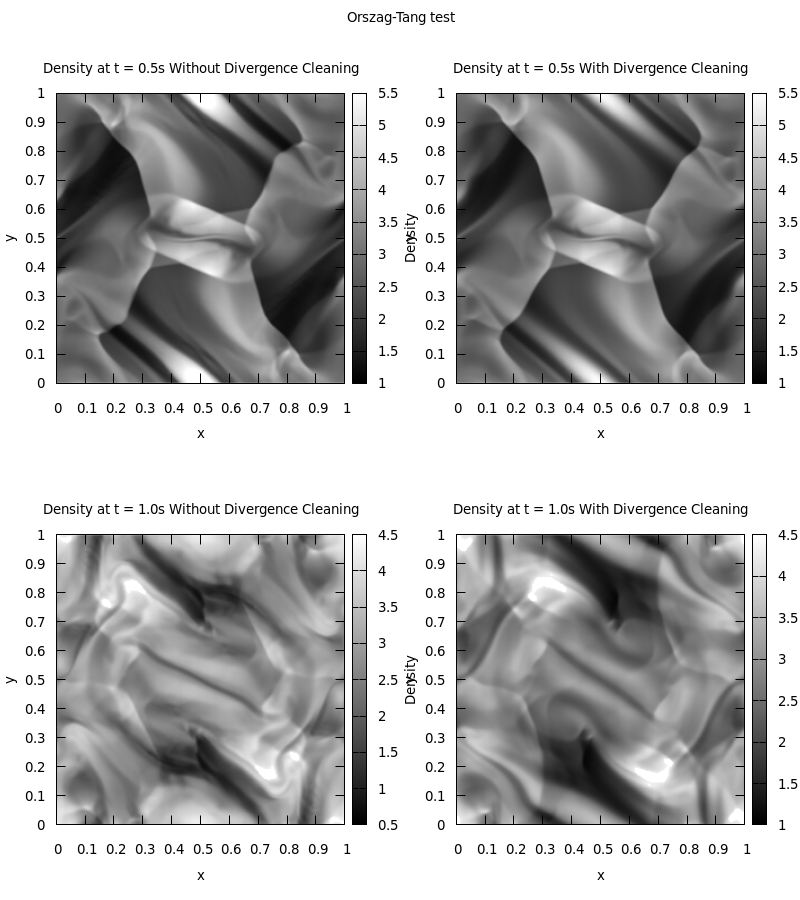
\includegraphics[width = \linewidth]{OrszagTang.png}
			\end{minipage}\\
			\vspace{0.2cm}
			\begin{minipage}{1.0\linewidth}
				\caption{Results of the Orszag-Tang test at $t=0.5$ (upper) and $t=1.0$ (lower), comparing the simulations with divergence cleaning (right) to the one without (left).}
				\label{fig:Orszag-Tang}
			\end{minipage}
		\end{figure}
		\vspace{0.6cm} 
		
		\begin{figure}
			\centering
			
			\begin{minipage}{0.60\textwidth}
				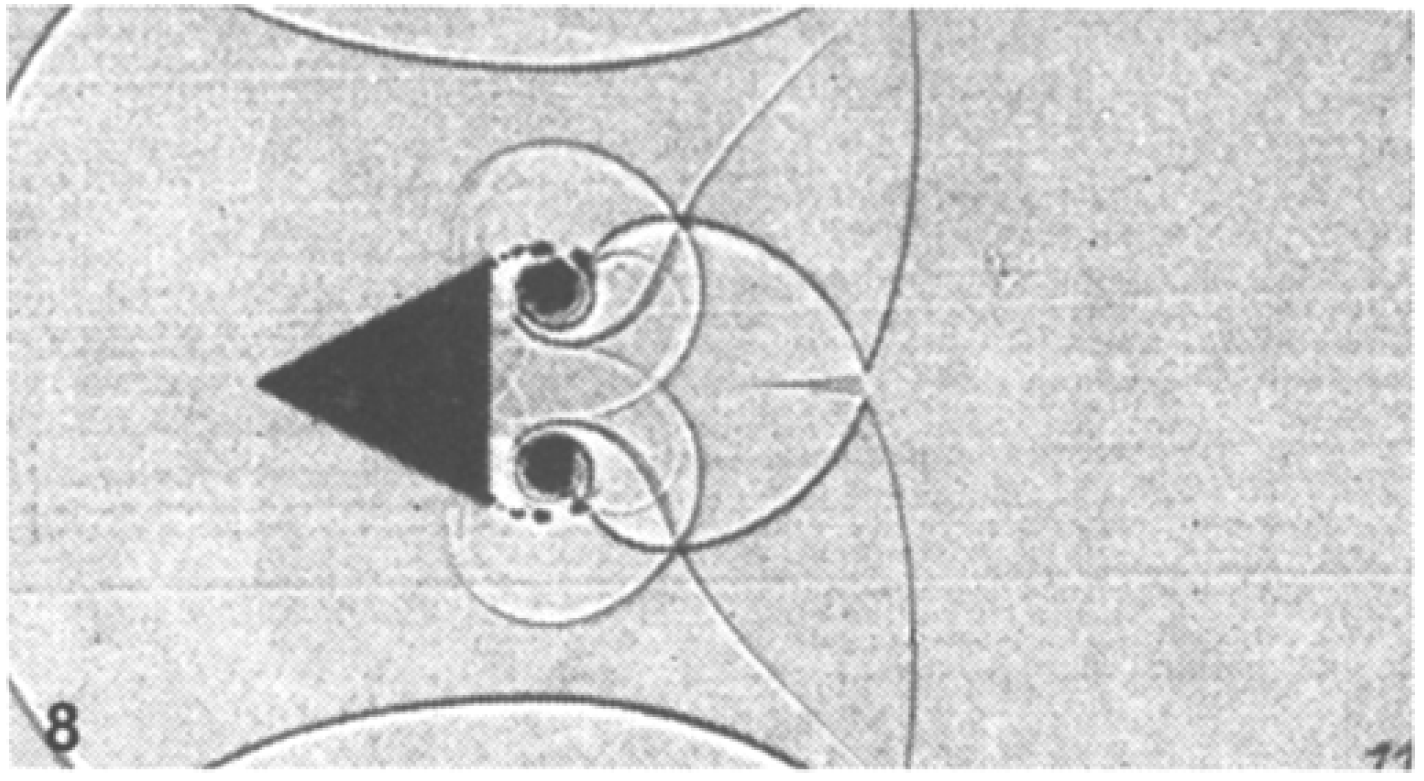
\includegraphics[width=\textwidth]{ShWe7.png}
			\end{minipage}
			\hspace{-3cm}
			\begin{minipage}{0.40\textwidth}
				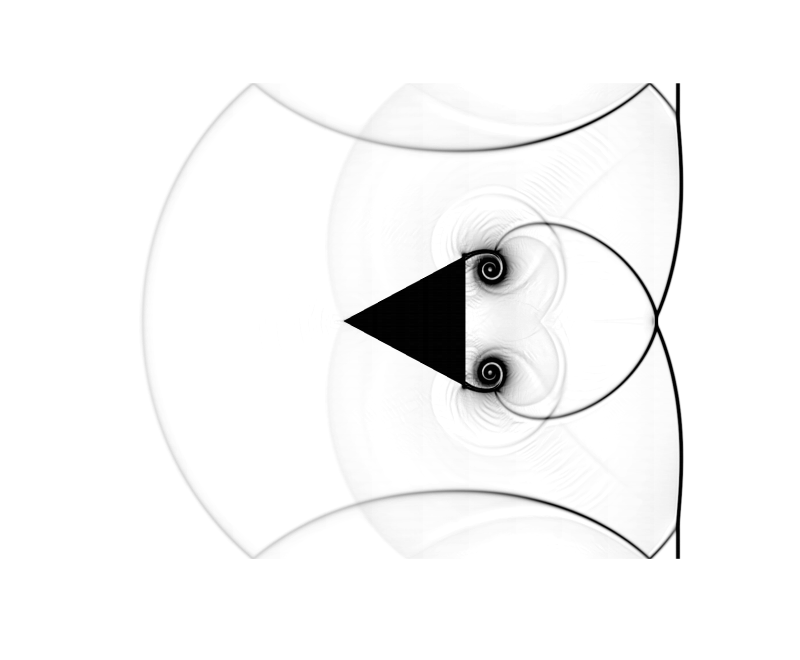
\includegraphics[width=\textwidth]{shock_wedge_2x_680.png}
			\end{minipage}
			\vspace{0.2cm}
			
			\begin{minipage}{0.45\textwidth}
				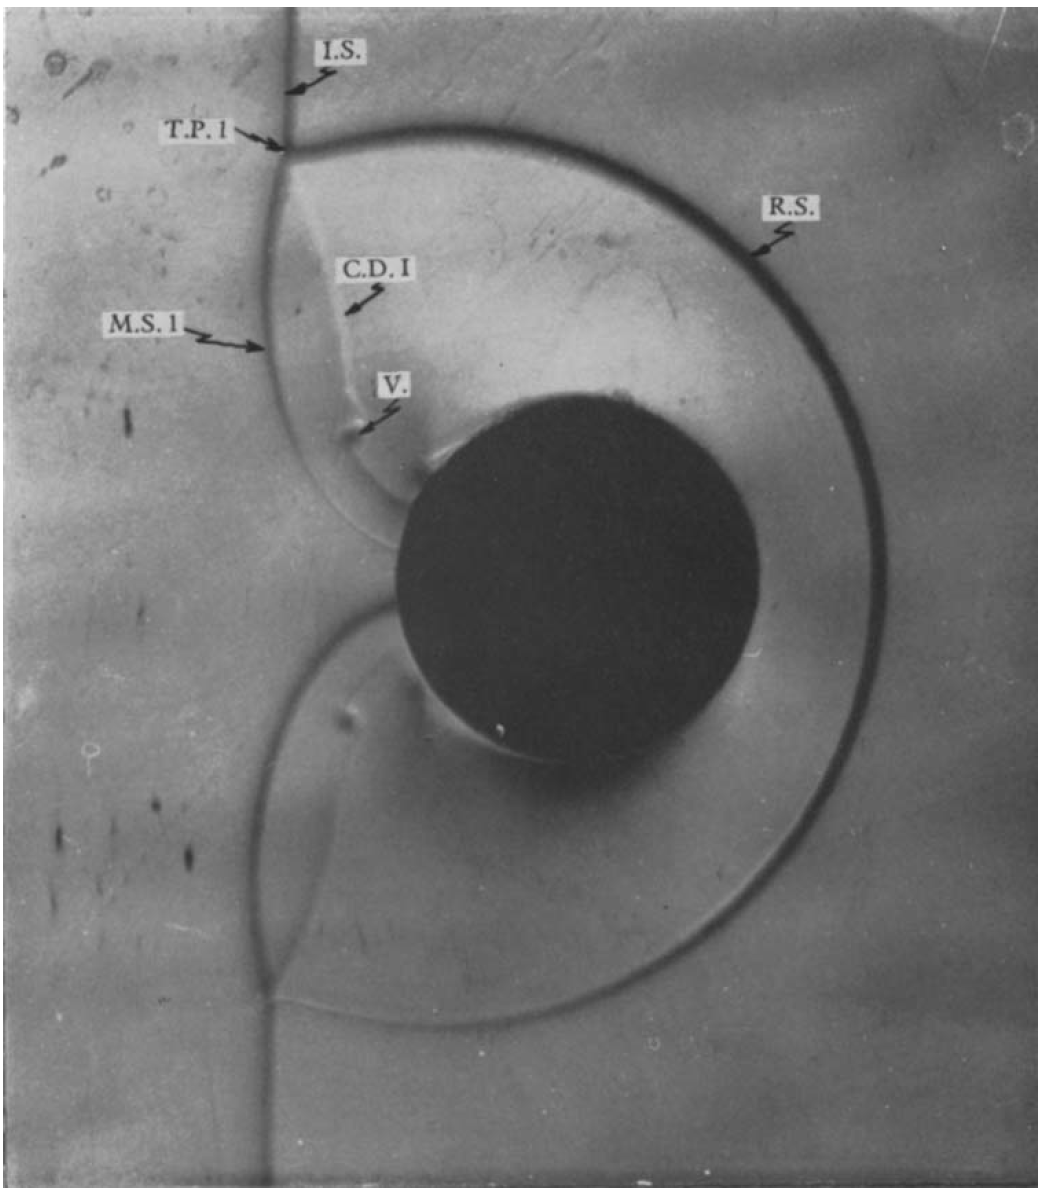
\includegraphics[width=\textwidth]{ShCy.png}
			\end{minipage}
			\hspace{-0.4cm}
			\begin{minipage}{0.4\textwidth}
				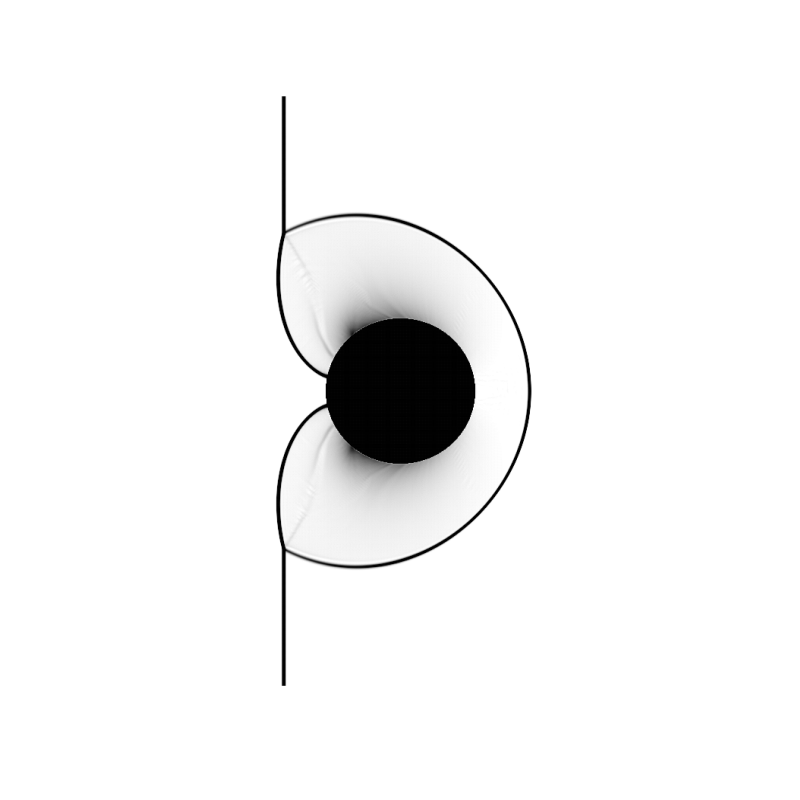
\includegraphics[width=\textwidth]{shock_cylinder_95.png}
			\end{minipage}
			\vspace{0.2cm}
			
			
			\begin{minipage}{1.0\textwidth}
				\caption{Schlieren plots for Shock diffraction over wedge or cylinder, comparing the results from simulations (right) to the experiment results (left).}
				\label{fig:shockwedge}
			\end{minipage}
			
		\end{figure}
	\end{minipage}
\end{block}
\vspace{-0.6cm}

\begin{block}{Validation for Resistive Wall}
\begin{minipage}{0.90\linewidth}
	\justifying
	The validation for resistive wall is adopted from a plasma cylindrical equilibrium test of Ferraro \textit{et al.} \cite{ferraro2016multi}. It is designed to model the resistive wall mode within a simplified straight cylindrical geometry. The Figure \ref{fig:InCy} demonstrates the initial state of cylindrical equilibrium test: 
	\vspace{0.2cm}
	\begin{figure}
	\begin{minipage}{1.0\textwidth}
		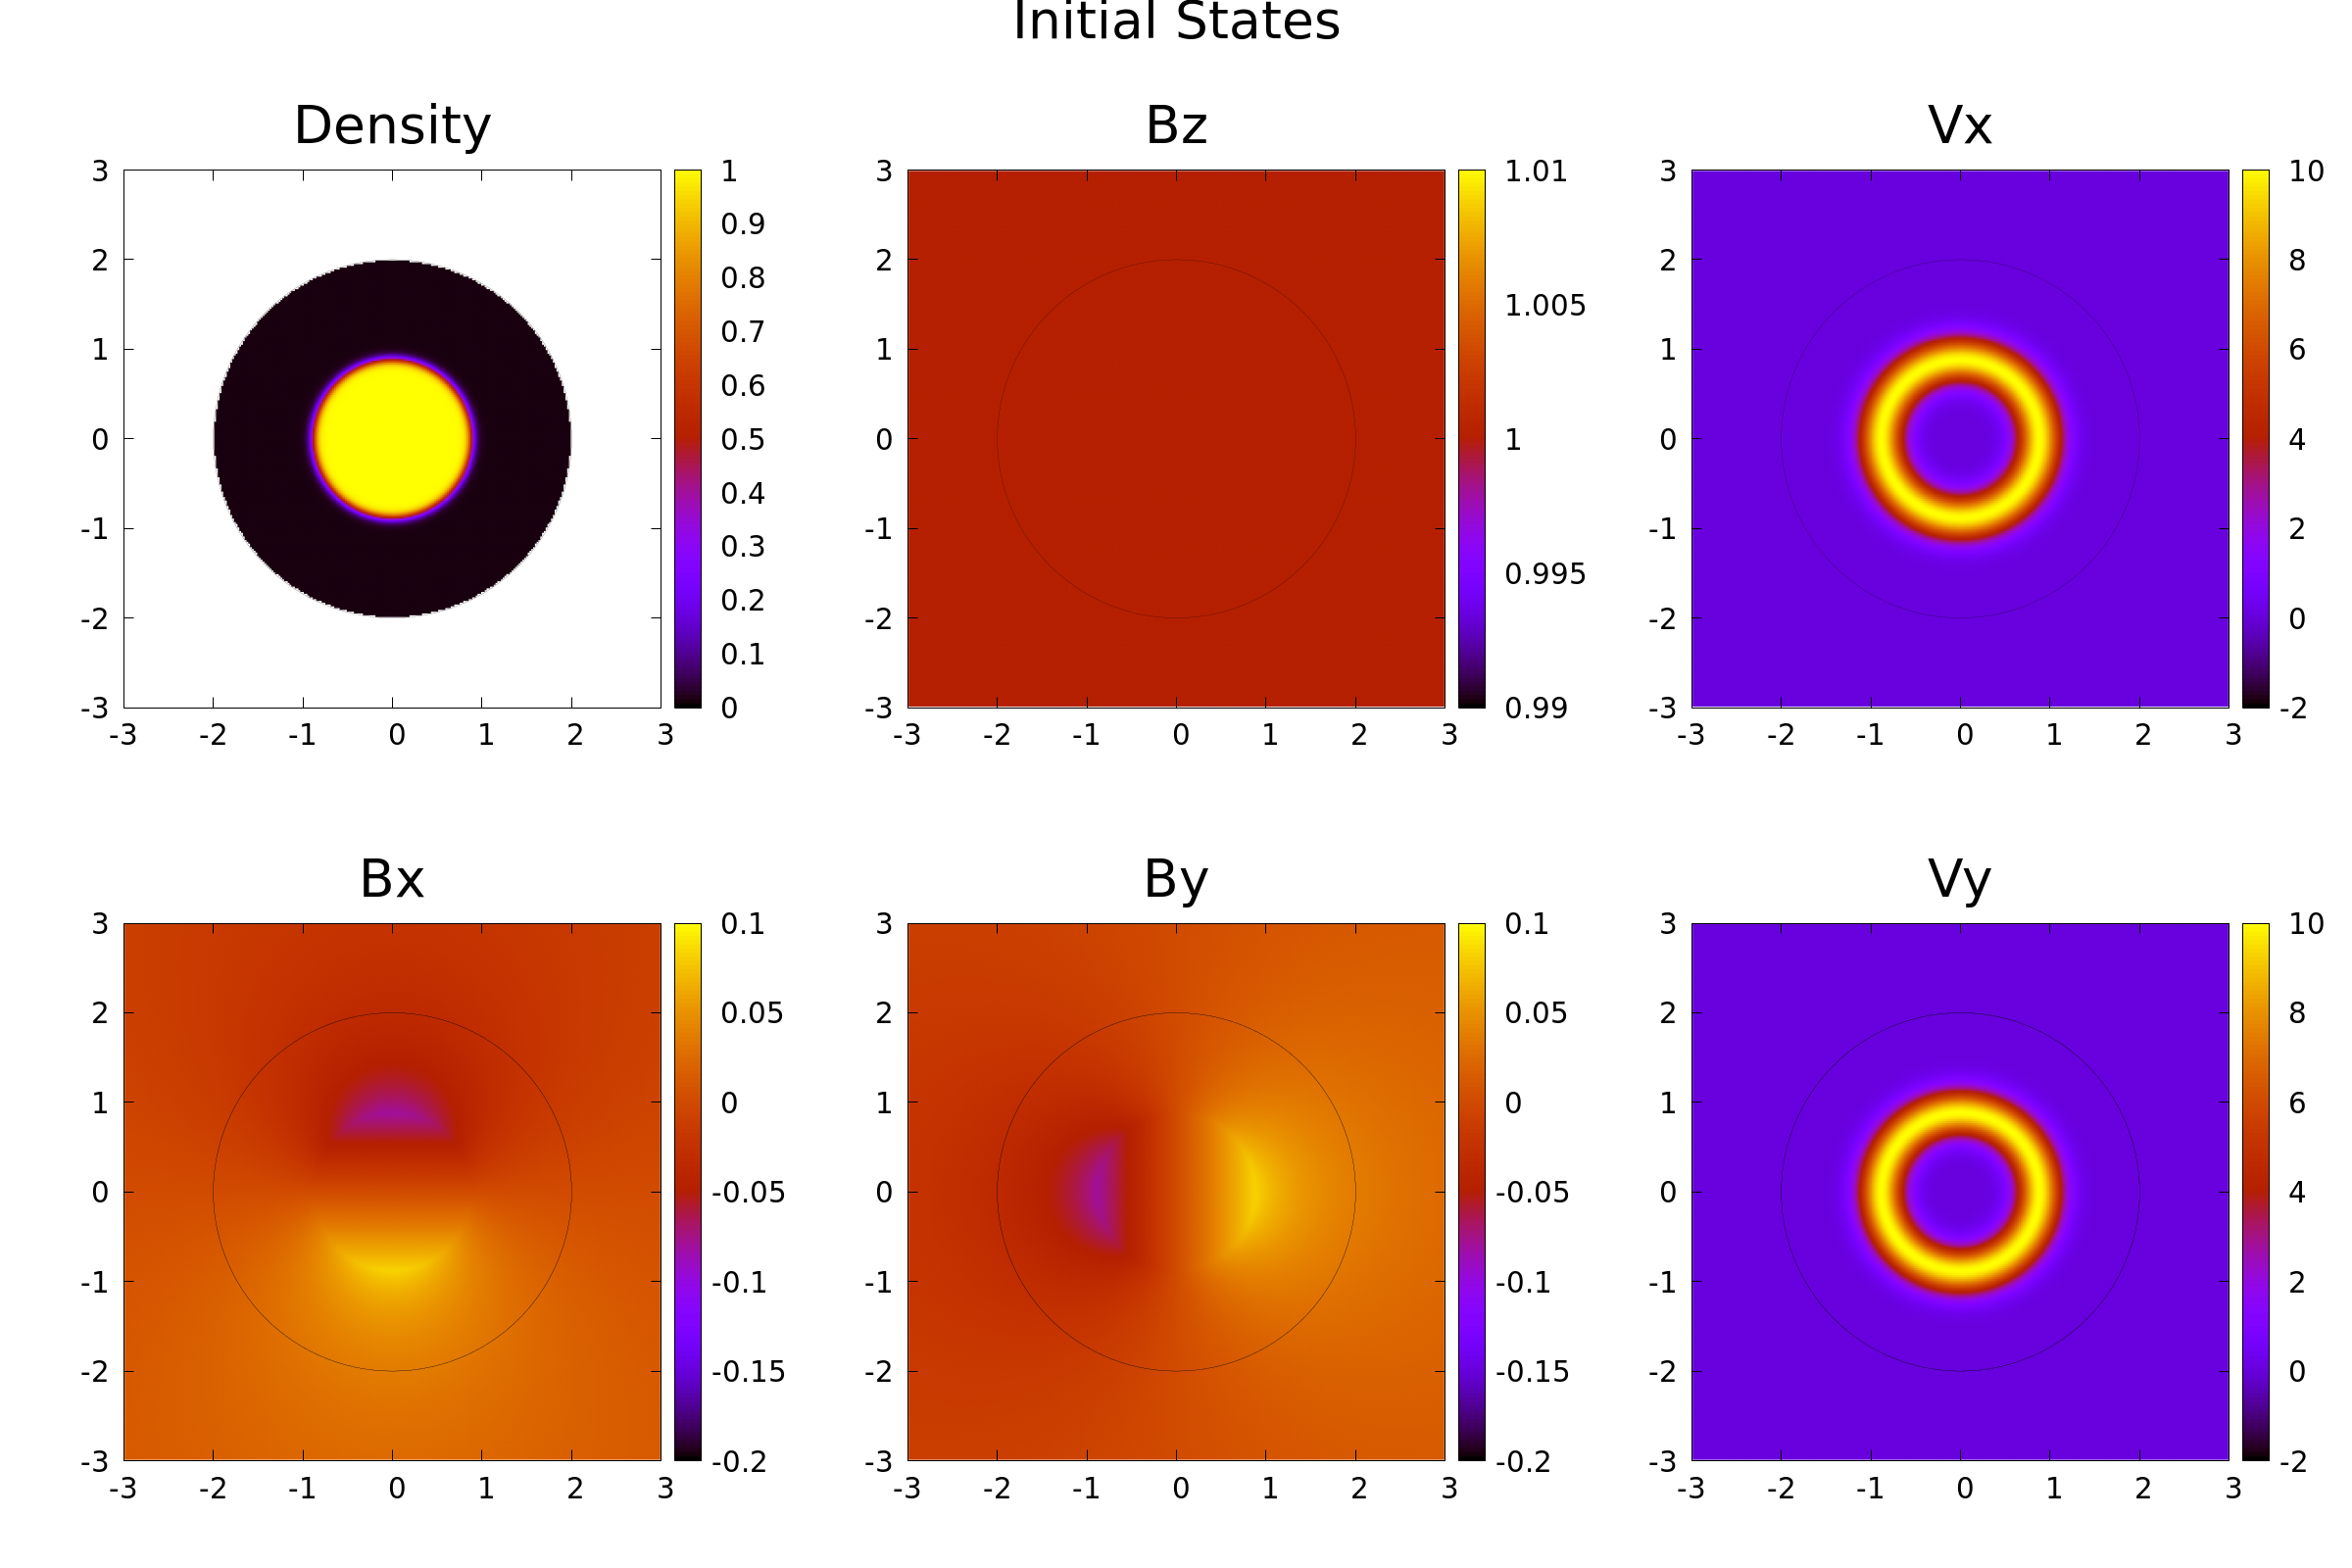
\includegraphics[width=\textwidth]{InitialCylindricalEquilibrium.png}
	\end{minipage}
	\vspace{0.2cm}
	
	\begin{minipage}{1.0\textwidth}
		\caption{Initial state of cylindrical equilibrium.}
		\label{fig:InCy}
	\end{minipage}
	\end{figure}
\end{minipage}
\end{block}

\end{textblock}

% Third column

\begin{textblock}{19.0}(39.0,7.5)
\begin{block}{Validation for Resistive Wall}
	\begin{minipage}{0.93\linewidth}
		\justifying
		The Figure \ref{fig:cy_mine} below demonstrate the results density and $B_z$ in the cylindrical equilibrium test. The resistive wall leads to a higher peak in $B_z$ showing a qualitative agreement with Chrysanthou's result \cite{chrysanthou2020} in Figure \ref{fig:cyBz_Maria}.
		\vspace{0.3cm}
		
		\begin{figure}
			\begin{minipage}{0.90\linewidth}
				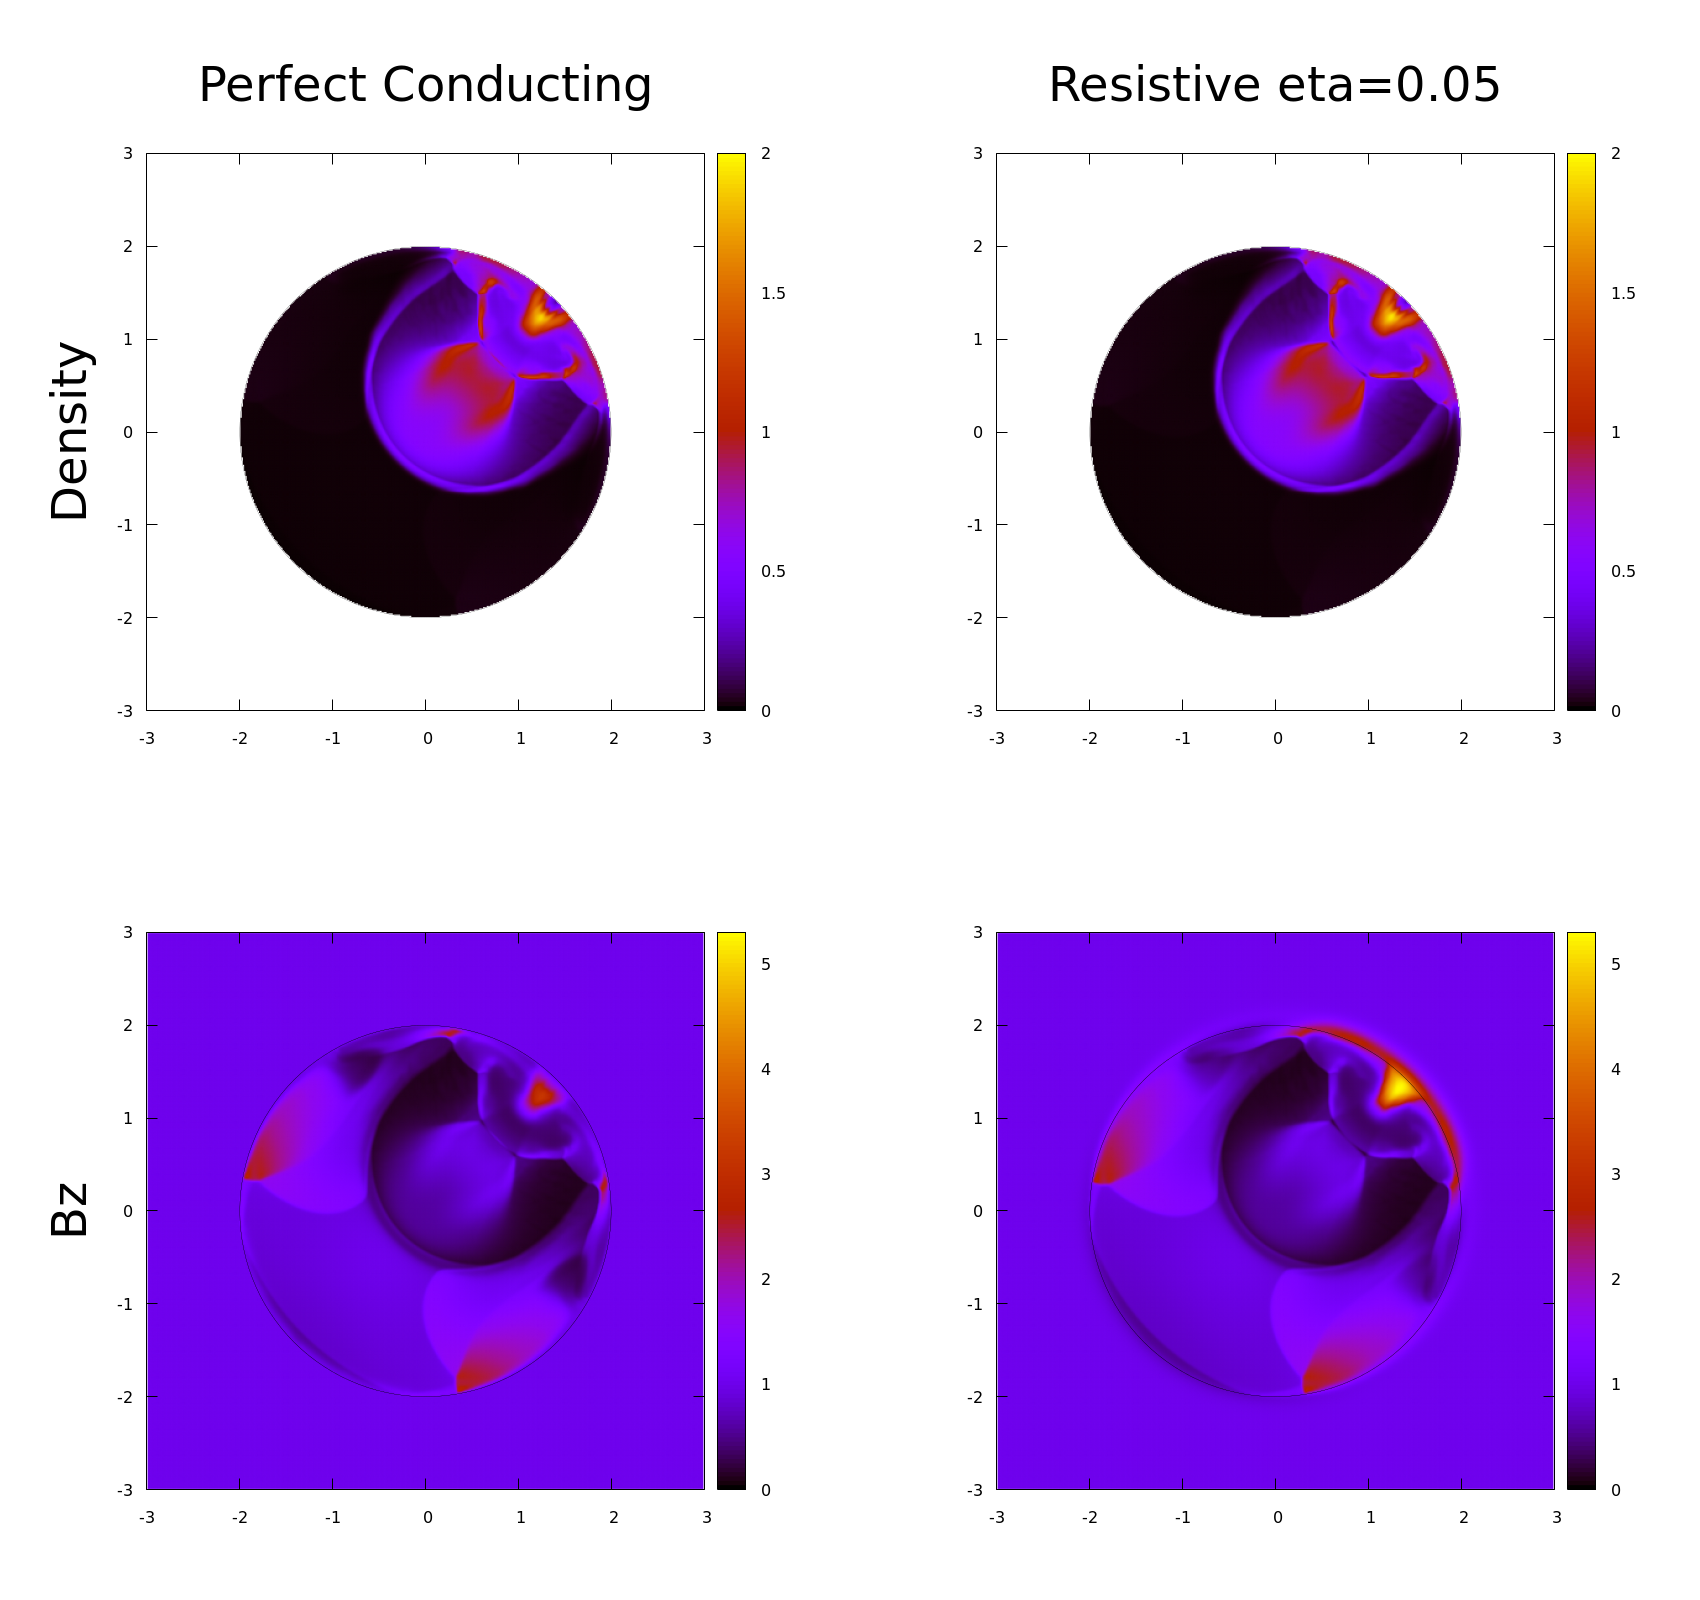
\includegraphics[width=\textwidth]{cylindricalEquilibrium.png}
			\end{minipage}
			
			\begin{minipage}{1.0\linewidth}
				\caption{Results of cylindrical equilibrium test comparing densities (upper) and $B_z$ (lower) with resistivities $\eta_{w}=0.0$ (left) and $\eta_{w}=0.05$ (right).}
				\label{fig:cy_mine}
			\end{minipage}
		\end{figure}
		\vspace{0.2cm}
		
		\begin{figure}
			\begin{minipage}{0.90\linewidth}
				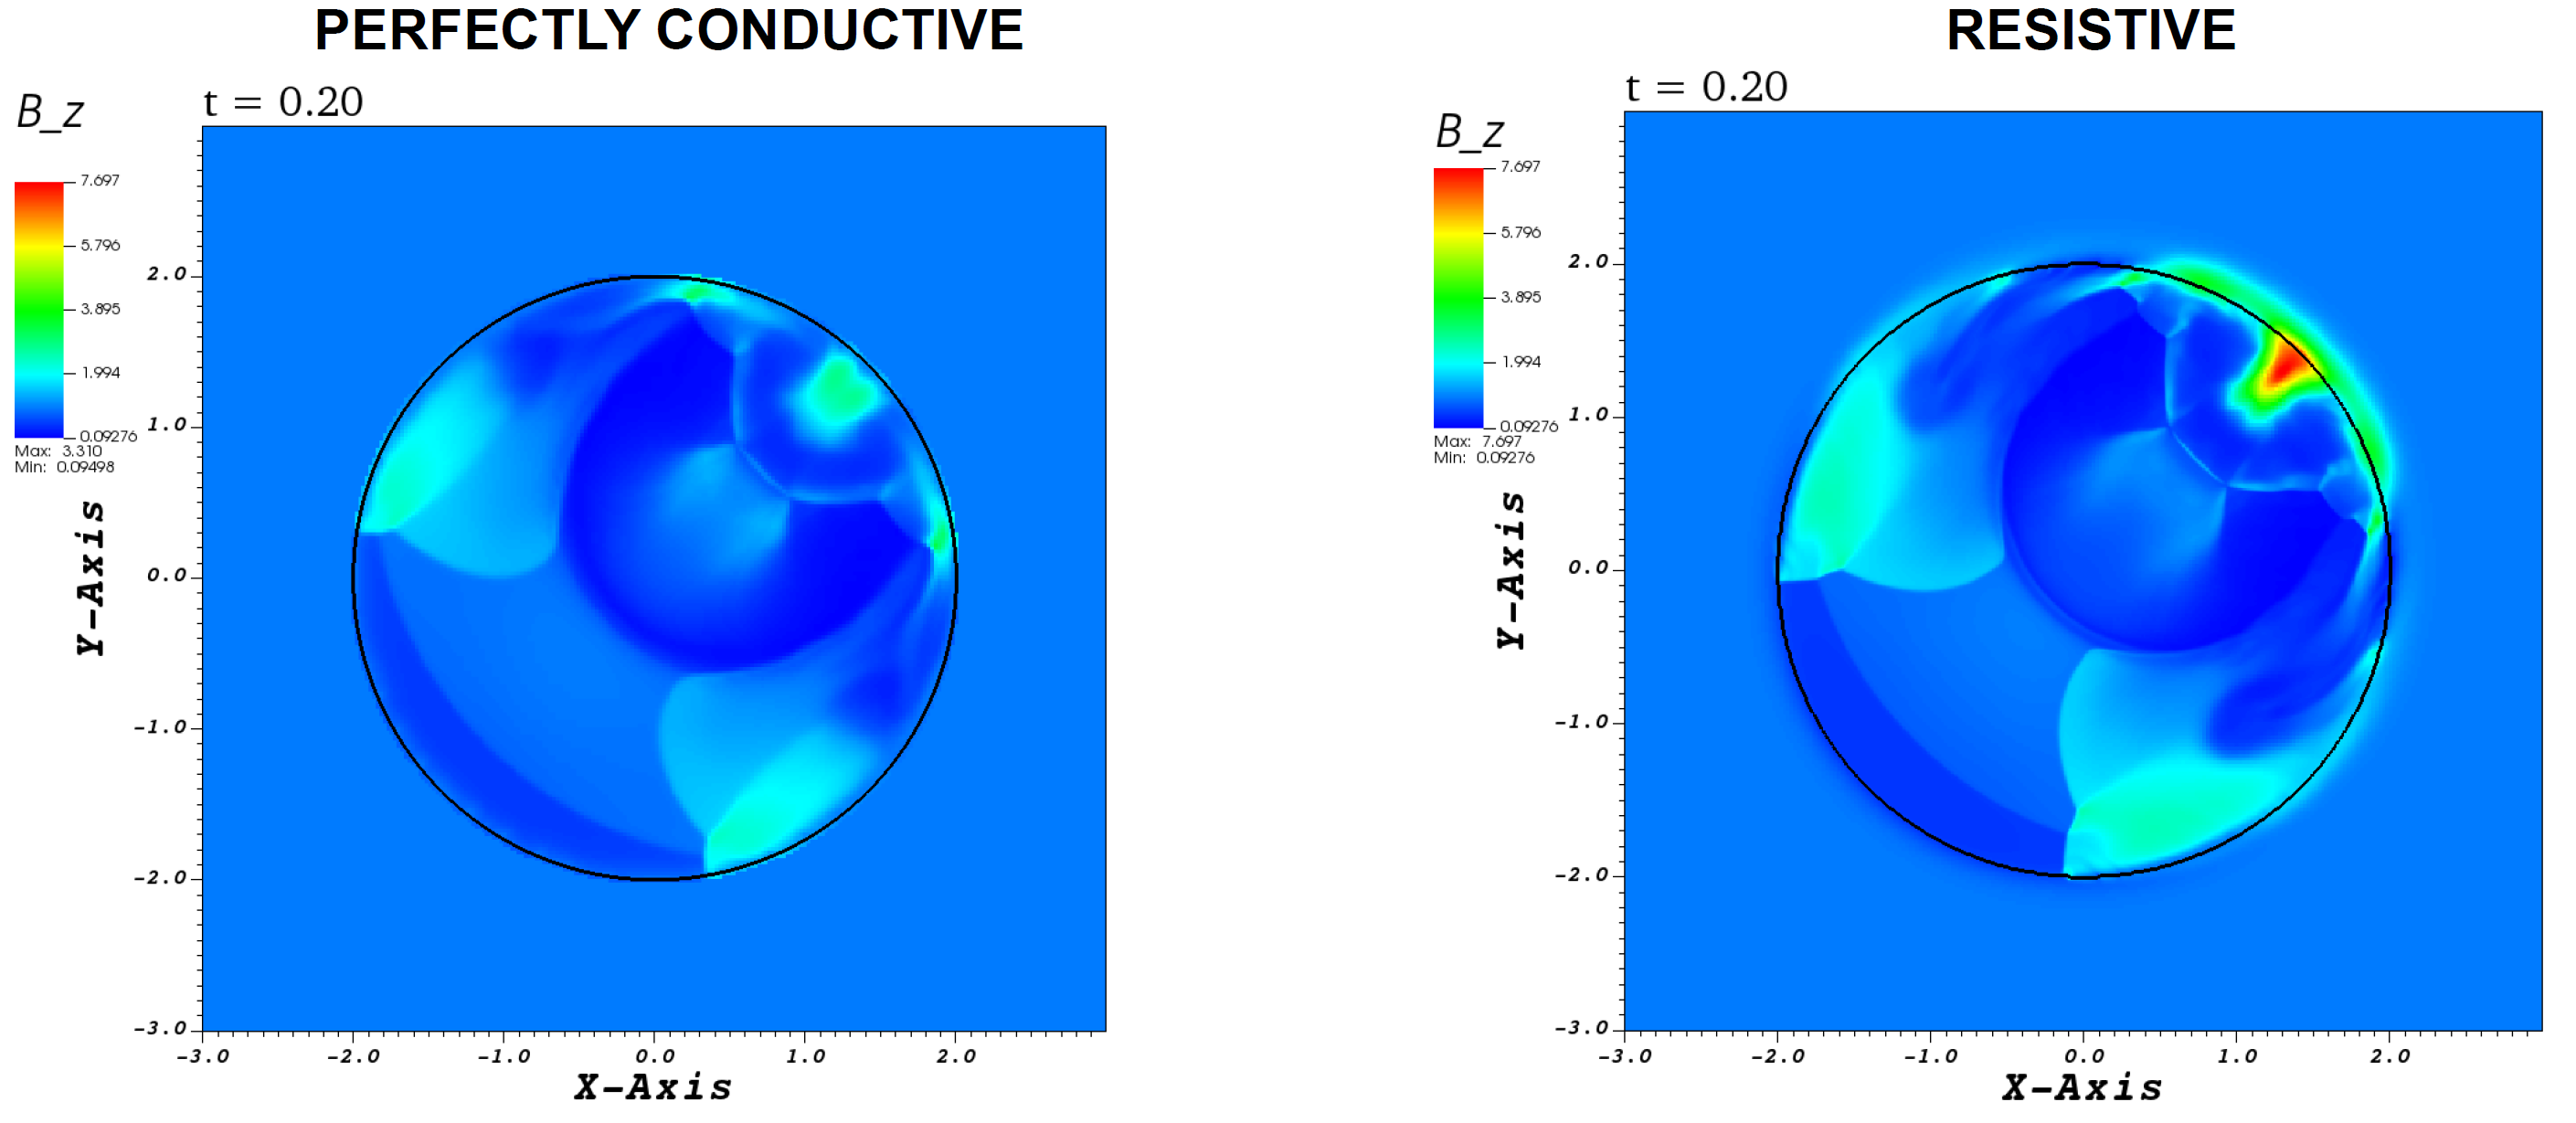
\includegraphics[width=\textwidth]{MariaResult2.png}
			\end{minipage}
			
			\begin{minipage}{1.0\linewidth}
				\caption{The $B_z$ result in Chrysanthou's test \cite{chrysanthou2020}.}
				\label{fig:cyBz_Maria}
			\end{minipage}
		\end{figure}
	\end{minipage}
\end{block}
\vspace{-0.5cm}	
	
\begin{block}{Plasma in Resistive Tokamak Vessel}
	\begin{minipage}{0.93\linewidth}
		\justifying
		The following graph shows density and $B_z$ in simulation within a resistive tokamak-shaped vessel. This figure is taken from the moment $t=0.2$ after the core dense plasma hitting the vessel wall with resistivity $\eta_w=0.05$. The interaction on magnetic field between plasma and vessel wall result in significant increase in $B_z$ on wall.\\
		\begin{figure}
			\begin{minipage}{0.48\linewidth}
				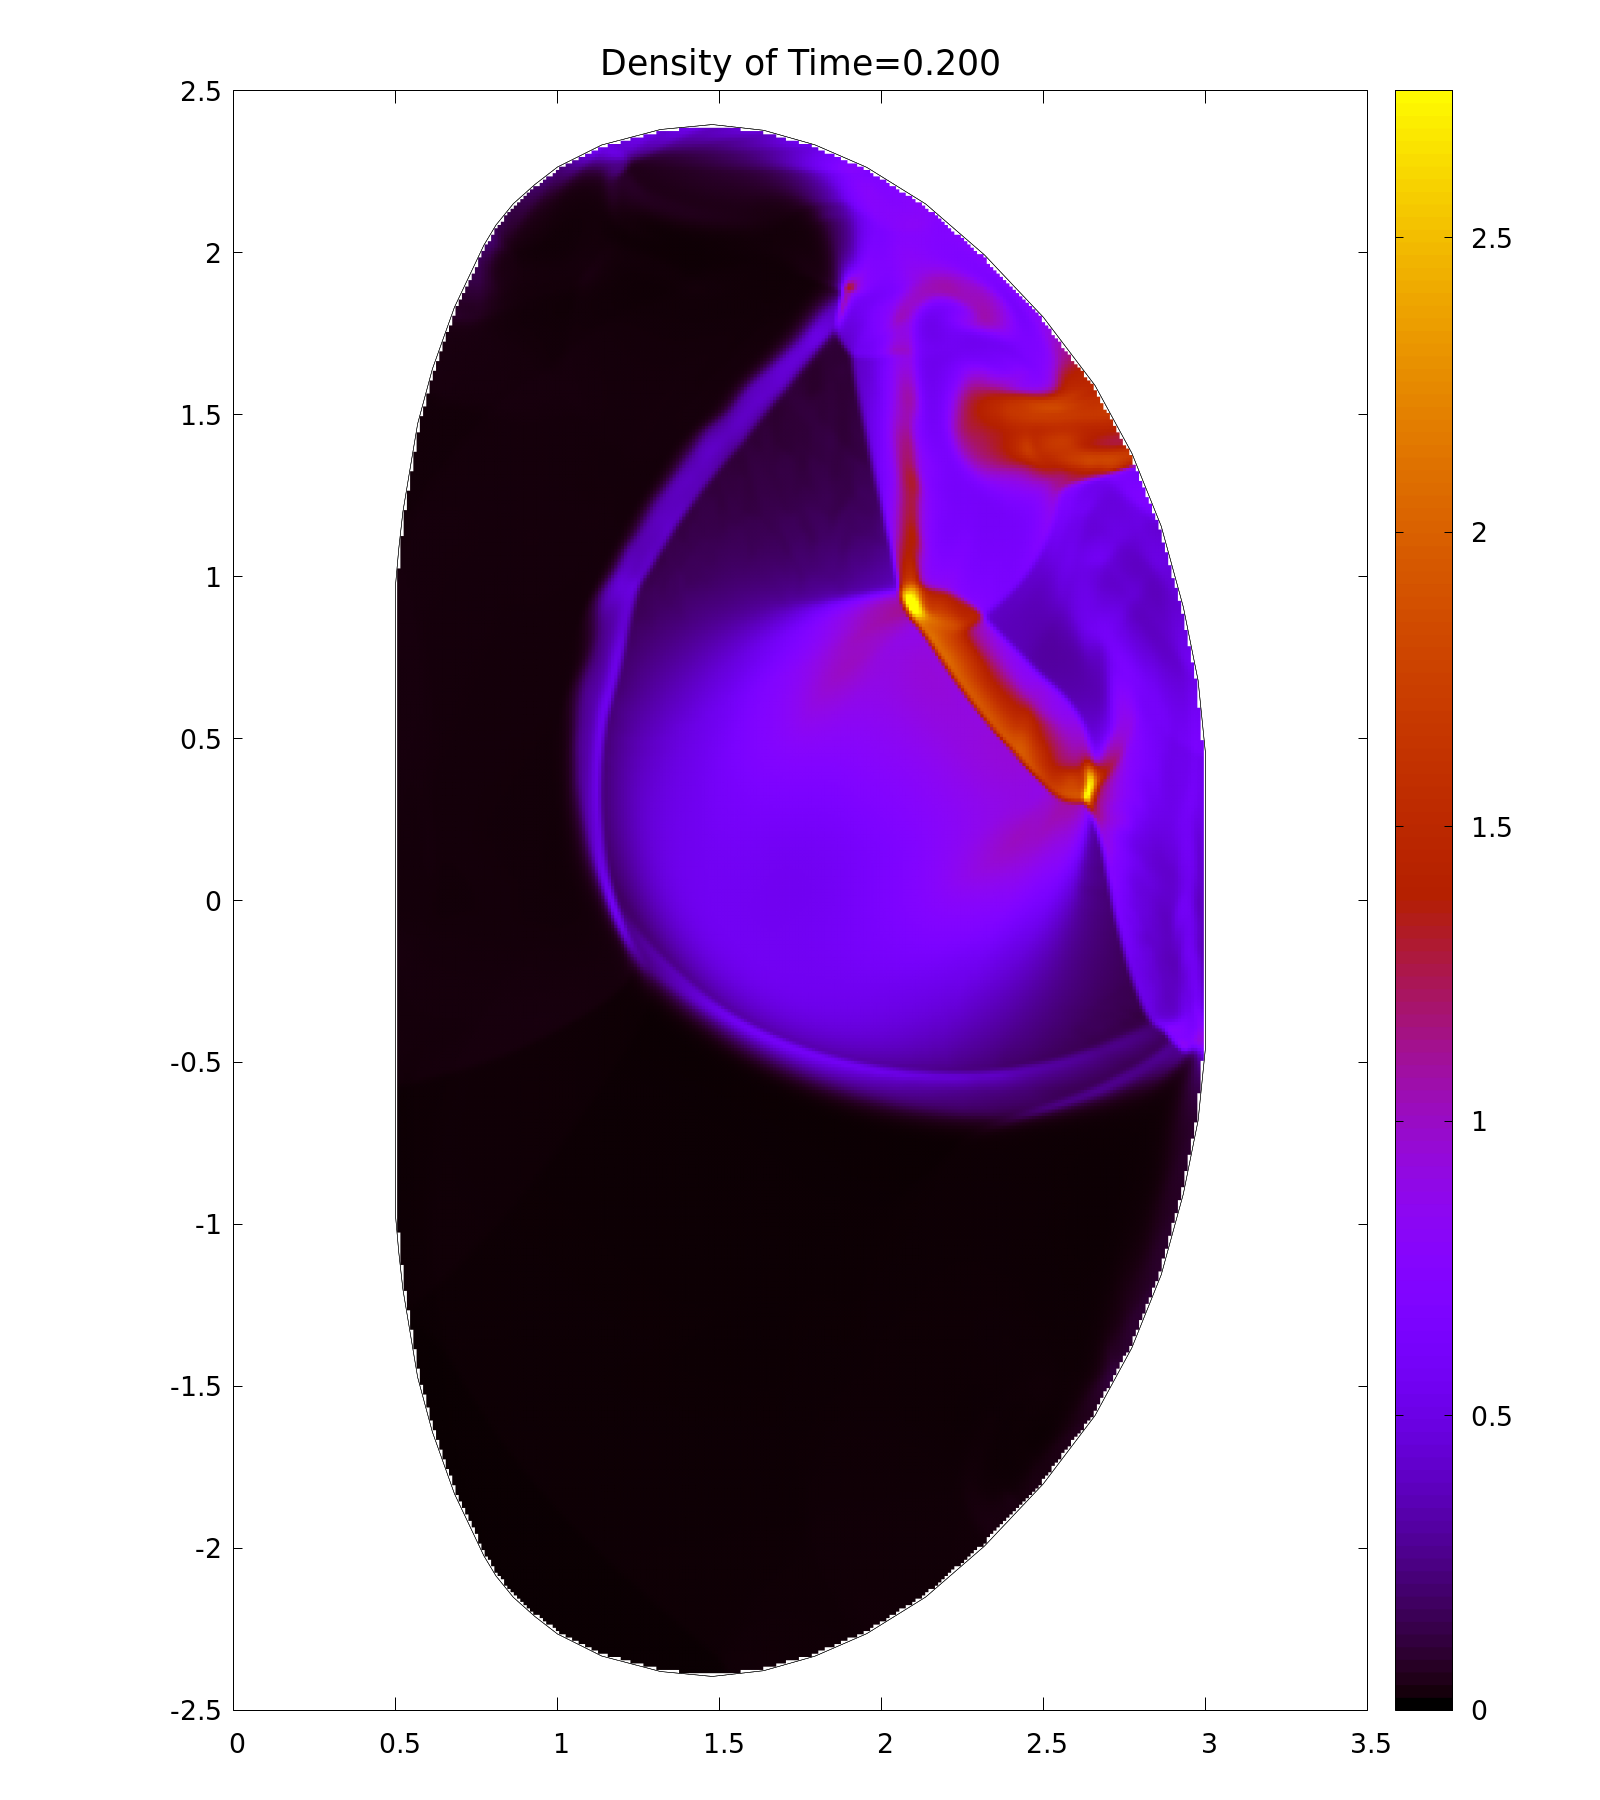
\includegraphics[width = \linewidth]{Poster_Density_100.png}
			\end{minipage}
			\hspace{-0.6cm}
			\begin{minipage}{0.48\linewidth}
				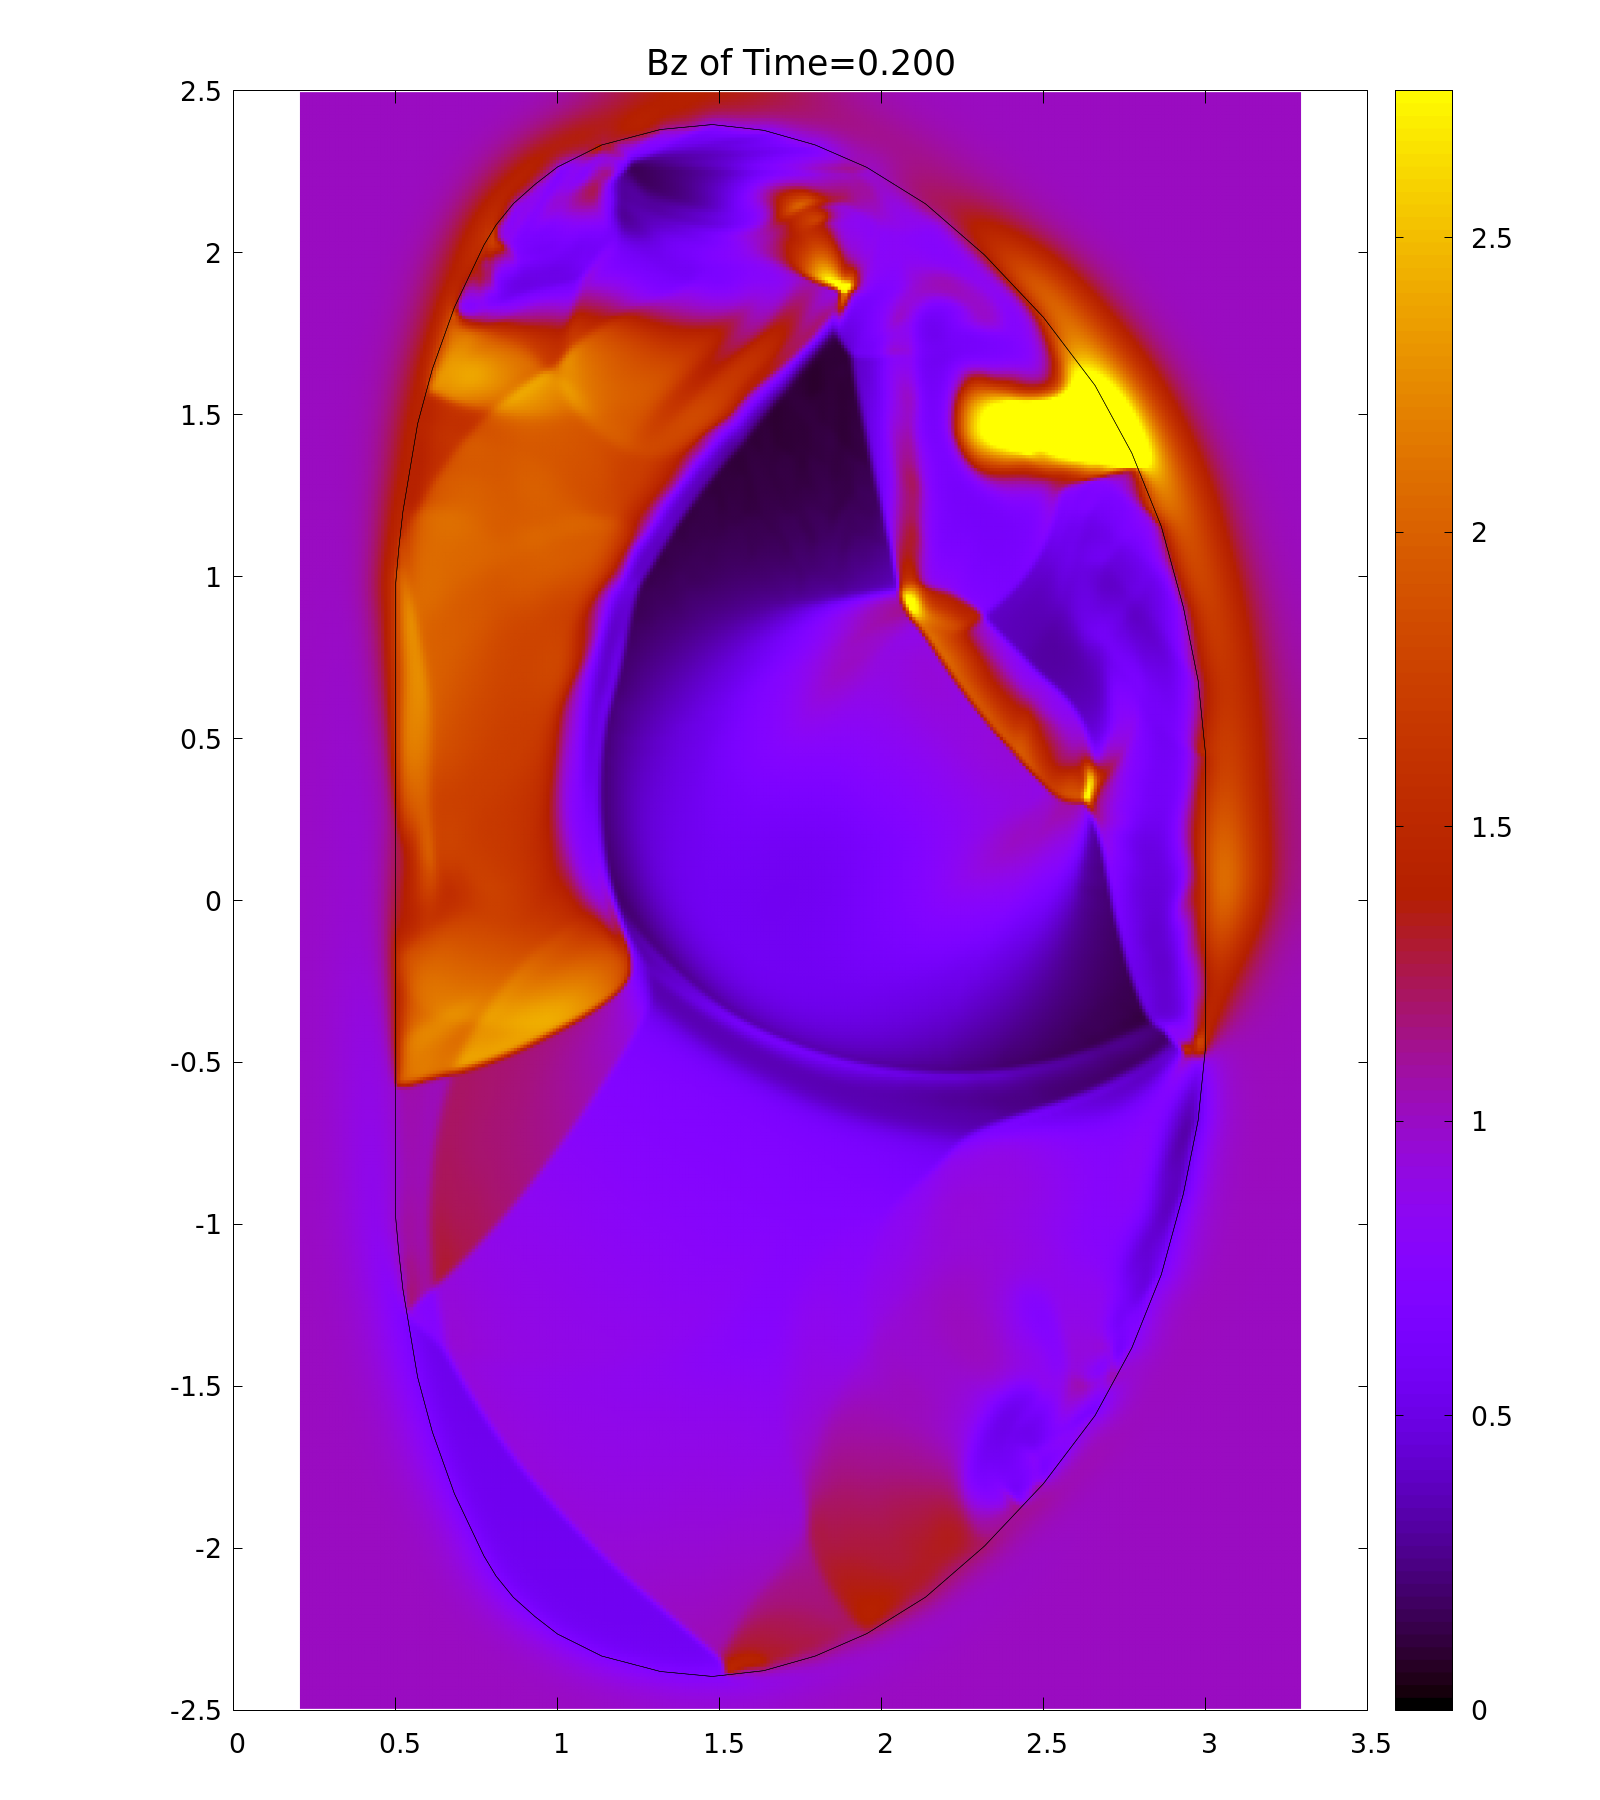
\includegraphics[width = \linewidth]{Poster_Bz_100.png}
			\end{minipage}\\
			\begin{minipage}{1.0\linewidth}
				\caption{Density (left) and $B_z$ (right) of plasma in a cylindrical equilibrium test within a tokamak-shaped vessel, outlined by a thin black line.}
			\end{minipage}
			\vspace{-0.2cm}
		\end{figure}
	\end{minipage}
\end{block}
\vspace{-0.5cm}

%\begin{block}{Consistent Equation}
%	After discussion on boundary condition consistency, a consistent equation across conditions is proposed
%	\begin{equation*}
%		\nabla^2\mathbf{B}=\frac{nq_e^2}{m\nu}\frac{\partial \mathbf{B}}{\partial t}-\frac{nq_e^2}{m\nu}e^{-\nu t}\frac{\partial \mathbf{B}}{\partial t}
%	\end{equation*}
%\end{block}

\begin{block}{References}
\begin{minipage}{0.95\linewidth}
     {     \printbibliography   % i.e. the references.bib file
     } 
\end{minipage}
\end{block}

\end{textblock}

\end{frame}
\end{document}
